% Options for packages loaded elsewhere
\PassOptionsToPackage{unicode}{hyperref}
\PassOptionsToPackage{hyphens}{url}
\PassOptionsToPackage{dvipsnames,svgnames,x11names}{xcolor}
%
\documentclass[
  letterpaper,
  DIV=11,
  numbers=noendperiod]{scrartcl}

\usepackage{amsmath,amssymb}
\usepackage{iftex}
\ifPDFTeX
  \usepackage[T1]{fontenc}
  \usepackage[utf8]{inputenc}
  \usepackage{textcomp} % provide euro and other symbols
\else % if luatex or xetex
  \usepackage{unicode-math}
  \defaultfontfeatures{Scale=MatchLowercase}
  \defaultfontfeatures[\rmfamily]{Ligatures=TeX,Scale=1}
\fi
\usepackage{lmodern}
\ifPDFTeX\else  
    % xetex/luatex font selection
\fi
% Use upquote if available, for straight quotes in verbatim environments
\IfFileExists{upquote.sty}{\usepackage{upquote}}{}
\IfFileExists{microtype.sty}{% use microtype if available
  \usepackage[]{microtype}
  \UseMicrotypeSet[protrusion]{basicmath} % disable protrusion for tt fonts
}{}
\makeatletter
\@ifundefined{KOMAClassName}{% if non-KOMA class
  \IfFileExists{parskip.sty}{%
    \usepackage{parskip}
  }{% else
    \setlength{\parindent}{0pt}
    \setlength{\parskip}{6pt plus 2pt minus 1pt}}
}{% if KOMA class
  \KOMAoptions{parskip=half}}
\makeatother
\usepackage{xcolor}
\setlength{\emergencystretch}{3em} % prevent overfull lines
\setcounter{secnumdepth}{-\maxdimen} % remove section numbering
% Make \paragraph and \subparagraph free-standing
\makeatletter
\ifx\paragraph\undefined\else
  \let\oldparagraph\paragraph
  \renewcommand{\paragraph}{
    \@ifstar
      \xxxParagraphStar
      \xxxParagraphNoStar
  }
  \newcommand{\xxxParagraphStar}[1]{\oldparagraph*{#1}\mbox{}}
  \newcommand{\xxxParagraphNoStar}[1]{\oldparagraph{#1}\mbox{}}
\fi
\ifx\subparagraph\undefined\else
  \let\oldsubparagraph\subparagraph
  \renewcommand{\subparagraph}{
    \@ifstar
      \xxxSubParagraphStar
      \xxxSubParagraphNoStar
  }
  \newcommand{\xxxSubParagraphStar}[1]{\oldsubparagraph*{#1}\mbox{}}
  \newcommand{\xxxSubParagraphNoStar}[1]{\oldsubparagraph{#1}\mbox{}}
\fi
\makeatother


\providecommand{\tightlist}{%
  \setlength{\itemsep}{0pt}\setlength{\parskip}{0pt}}\usepackage{longtable,booktabs,array}
\usepackage{calc} % for calculating minipage widths
% Correct order of tables after \paragraph or \subparagraph
\usepackage{etoolbox}
\makeatletter
\patchcmd\longtable{\par}{\if@noskipsec\mbox{}\fi\par}{}{}
\makeatother
% Allow footnotes in longtable head/foot
\IfFileExists{footnotehyper.sty}{\usepackage{footnotehyper}}{\usepackage{footnote}}
\makesavenoteenv{longtable}
\usepackage{graphicx}
\makeatletter
\def\maxwidth{\ifdim\Gin@nat@width>\linewidth\linewidth\else\Gin@nat@width\fi}
\def\maxheight{\ifdim\Gin@nat@height>\textheight\textheight\else\Gin@nat@height\fi}
\makeatother
% Scale images if necessary, so that they will not overflow the page
% margins by default, and it is still possible to overwrite the defaults
% using explicit options in \includegraphics[width, height, ...]{}
\setkeys{Gin}{width=\maxwidth,height=\maxheight,keepaspectratio}
% Set default figure placement to htbp
\makeatletter
\def\fps@figure{htbp}
\makeatother
% definitions for citeproc citations
\NewDocumentCommand\citeproctext{}{}
\NewDocumentCommand\citeproc{mm}{%
  \begingroup\def\citeproctext{#2}\cite{#1}\endgroup}
\makeatletter
 % allow citations to break across lines
 \let\@cite@ofmt\@firstofone
 % avoid brackets around text for \cite:
 \def\@biblabel#1{}
 \def\@cite#1#2{{#1\if@tempswa , #2\fi}}
\makeatother
\newlength{\cslhangindent}
\setlength{\cslhangindent}{1.5em}
\newlength{\csllabelwidth}
\setlength{\csllabelwidth}{3em}
\newenvironment{CSLReferences}[2] % #1 hanging-indent, #2 entry-spacing
 {\begin{list}{}{%
  \setlength{\itemindent}{0pt}
  \setlength{\leftmargin}{0pt}
  \setlength{\parsep}{0pt}
  % turn on hanging indent if param 1 is 1
  \ifodd #1
   \setlength{\leftmargin}{\cslhangindent}
   \setlength{\itemindent}{-1\cslhangindent}
  \fi
  % set entry spacing
  \setlength{\itemsep}{#2\baselineskip}}}
 {\end{list}}
\usepackage{calc}
\newcommand{\CSLBlock}[1]{\hfill\break\parbox[t]{\linewidth}{\strut\ignorespaces#1\strut}}
\newcommand{\CSLLeftMargin}[1]{\parbox[t]{\csllabelwidth}{\strut#1\strut}}
\newcommand{\CSLRightInline}[1]{\parbox[t]{\linewidth - \csllabelwidth}{\strut#1\strut}}
\newcommand{\CSLIndent}[1]{\hspace{\cslhangindent}#1}

\KOMAoption{captions}{tableheading}
\makeatletter
\@ifpackageloaded{caption}{}{\usepackage{caption}}
\AtBeginDocument{%
\ifdefined\contentsname
  \renewcommand*\contentsname{Table of contents}
\else
  \newcommand\contentsname{Table of contents}
\fi
\ifdefined\listfigurename
  \renewcommand*\listfigurename{List of Figures}
\else
  \newcommand\listfigurename{List of Figures}
\fi
\ifdefined\listtablename
  \renewcommand*\listtablename{List of Tables}
\else
  \newcommand\listtablename{List of Tables}
\fi
\ifdefined\figurename
  \renewcommand*\figurename{Figure}
\else
  \newcommand\figurename{Figure}
\fi
\ifdefined\tablename
  \renewcommand*\tablename{Table}
\else
  \newcommand\tablename{Table}
\fi
}
\@ifpackageloaded{float}{}{\usepackage{float}}
\floatstyle{ruled}
\@ifundefined{c@chapter}{\newfloat{codelisting}{h}{lop}}{\newfloat{codelisting}{h}{lop}[chapter]}
\floatname{codelisting}{Listing}
\newcommand*\listoflistings{\listof{codelisting}{List of Listings}}
\makeatother
\makeatletter
\makeatother
\makeatletter
\@ifpackageloaded{caption}{}{\usepackage{caption}}
\@ifpackageloaded{subcaption}{}{\usepackage{subcaption}}
\makeatother

\ifLuaTeX
  \usepackage{selnolig}  % disable illegal ligatures
\fi
\usepackage{bookmark}

\IfFileExists{xurl.sty}{\usepackage{xurl}}{} % add URL line breaks if available
\urlstyle{same} % disable monospaced font for URLs
\hypersetup{
  pdftitle={INDY Notes \& Simulations},
  colorlinks=true,
  linkcolor={blue},
  filecolor={Maroon},
  citecolor={Blue},
  urlcolor={Blue},
  pdfcreator={LaTeX via pandoc}}


\title{INDY Notes \& Simulations}
\author{}
\date{}

\begin{document}
\maketitle


\section{Page Navigation}\label{page-navigation}

\begin{enumerate}
\def\labelenumi{\arabic{enumi}.}
\tightlist
\item
  Vincent Tassion
\item
  Metric Backbone \& Spectral Clustering Simulations
\item
  Graph with Gaussian clusters \& ABBE prediction
\item
  Proof of THM 2.1
\item
  Instructions to deploy website
\item
  First Passage Percolation On Inhomogeneous Random Graphs
\item
  Module dependencies
\item
  hybrid graph μ fixed n\_neighbors varying
\item
  20241107 presentation
\end{enumerate}

\section{1}\label{section}

\subsection{Row}\label{row}

\subsubsection{Percolation Demo}\label{percolation-demo}

\paragraph{}\label{section-1}

\phantomsection\label{input_selects_1}
\phantomsection\label{input_selects_1-1}
\begin{verbatim}
<h2>Percolation Demo</h2>
\end{verbatim}

\phantomsection\label{input_selects_1-2}
\begin{verbatim}
<div class="form-group shiny-input-container" style="width:10;">
  <label class="control-label" id="p-label" for="p">Probability:</label>
  <div>
    <select class="shiny-input-select form-select" id="p">      <option value="0.01">0.01</option>
      <option value="0.02">0.02</option>
      <option value="0.03">0.03</option>
      <option value="0.04">0.04</option>
      <option value="0.05">0.05</option>
      <option value="0.06">0.06</option>
      <option value="0.07">0.07</option>
      <option value="0.08">0.08</option>
      <option value="0.09">0.09</option>
      <option value="0.1">0.1</option>
      <option value="0.11">0.11</option>
      <option value="0.12">0.12</option>
      <option value="0.13">0.13</option>
      <option value="0.14">0.14</option>
      <option value="0.15">0.15</option>
      <option value="0.16">0.16</option>
      <option value="0.17">0.17</option>
      <option value="0.18">0.18</option>
      <option value="0.19">0.19</option>
      <option value="0.2">0.2</option>
      <option value="0.21">0.21</option>
      <option value="0.22">0.22</option>
      <option value="0.23">0.23</option>
      <option value="0.24">0.24</option>
      <option value="0.25">0.25</option>
      <option value="0.26">0.26</option>
      <option value="0.27">0.27</option>
      <option value="0.28">0.28</option>
      <option value="0.29">0.29</option>
      <option value="0.3">0.3</option>
      <option value="0.31">0.31</option>
      <option value="0.32">0.32</option>
      <option value="0.33">0.33</option>
      <option value="0.34">0.34</option>
      <option value="0.35">0.35</option>
      <option value="0.36">0.36</option>
      <option value="0.37">0.37</option>
      <option value="0.38">0.38</option>
      <option value="0.39">0.39</option>
      <option value="0.4">0.4</option>
      <option value="0.41">0.41</option>
      <option value="0.42">0.42</option>
      <option value="0.43">0.43</option>
      <option value="0.44">0.44</option>
      <option value="0.45">0.45</option>
      <option value="0.46">0.46</option>
      <option value="0.47">0.47</option>
      <option value="0.48">0.48</option>
      <option value="0.49">0.49</option>
      <option value="0.5" selected="">0.5</option>
      <option value="0.51">0.51</option>
      <option value="0.52">0.52</option>
      <option value="0.53">0.53</option>
      <option value="0.54">0.54</option>
      <option value="0.55">0.55</option>
      <option value="0.56">0.56</option>
      <option value="0.57">0.57</option>
      <option value="0.58">0.58</option>
      <option value="0.59">0.59</option>
      <option value="0.6">0.6</option>
      <option value="0.61">0.61</option>
      <option value="0.62">0.62</option>
      <option value="0.63">0.63</option>
      <option value="0.64">0.64</option>
      <option value="0.65">0.65</option>
      <option value="0.66">0.66</option>
      <option value="0.67">0.67</option>
      <option value="0.68">0.68</option>
      <option value="0.69">0.69</option>
      <option value="0.7">0.7</option>
      <option value="0.71">0.71</option>
      <option value="0.72">0.72</option>
      <option value="0.73">0.73</option>
      <option value="0.74">0.74</option>
      <option value="0.75">0.75</option>
      <option value="0.76">0.76</option>
      <option value="0.77">0.77</option>
      <option value="0.78">0.78</option>
      <option value="0.79">0.79</option>
      <option value="0.8">0.8</option>
      <option value="0.81">0.81</option>
      <option value="0.82">0.82</option>
      <option value="0.83">0.83</option>
      <option value="0.84">0.84</option>
      <option value="0.85">0.85</option>
      <option value="0.86">0.86</option>
      <option value="0.87">0.87</option>
      <option value="0.88">0.88</option>
      <option value="0.89">0.89</option>
      <option value="0.9">0.9</option>
      <option value="0.91">0.91</option>
      <option value="0.92">0.92</option>
      <option value="0.93">0.93</option>
      <option value="0.94">0.94</option>
      <option value="0.95">0.95</option>
      <option value="0.96">0.96</option>
      <option value="0.97">0.97</option>
      <option value="0.98">0.98</option>
      <option value="0.99">0.99</option></select>
  </div>
</div>
\end{verbatim}

\phantomsection\label{input_selects_1-3}
\begin{verbatim}
<div class="form-group shiny-input-container">
  <label class="control-label" id="grid_size-label" for="grid_size">Number of nodes in each dimension:</label>
  <div>
    <select class="shiny-input-select form-select" id="grid_size">      <option value="2">2</option>
      <option value="3">3</option>
      <option value="4">4</option>
      <option value="5">5</option>
      <option value="6">6</option>
      <option value="7">7</option>
      <option value="8">8</option>
      <option value="9">9</option>
      <option value="10" selected="">10</option>
      <option value="11">11</option>
      <option value="12">12</option>
      <option value="13">13</option>
      <option value="14">14</option>
      <option value="15">15</option>
      <option value="16">16</option>
      <option value="17">17</option>
      <option value="18">18</option>
      <option value="19">19</option>
      <option value="20">20</option>
      <option value="21">21</option>
      <option value="22">22</option>
      <option value="23">23</option>
      <option value="24">24</option>
      <option value="25">25</option>
      <option value="26">26</option>
      <option value="27">27</option>
      <option value="28">28</option>
      <option value="29">29</option>
      <option value="30">30</option>
      <option value="31">31</option>
      <option value="32">32</option>
      <option value="33">33</option>
      <option value="34">34</option>
      <option value="35">35</option>
      <option value="36">36</option>
      <option value="37">37</option>
      <option value="38">38</option>
      <option value="39">39</option>
      <option value="40">40</option>
      <option value="41">41</option>
      <option value="42">42</option>
      <option value="43">43</option>
      <option value="44">44</option>
      <option value="45">45</option>
      <option value="46">46</option>
      <option value="47">47</option>
      <option value="48">48</option>
      <option value="49">49</option>
      <option value="50">50</option>
      <option value="51">51</option>
      <option value="52">52</option>
      <option value="53">53</option>
      <option value="54">54</option>
      <option value="55">55</option>
      <option value="56">56</option>
      <option value="57">57</option>
      <option value="58">58</option>
      <option value="59">59</option>
      <option value="60">60</option>
      <option value="61">61</option>
      <option value="62">62</option>
      <option value="63">63</option>
      <option value="64">64</option>
      <option value="65">65</option>
      <option value="66">66</option>
      <option value="67">67</option>
      <option value="68">68</option>
      <option value="69">69</option>
      <option value="70">70</option>
      <option value="71">71</option>
      <option value="72">72</option>
      <option value="73">73</option>
      <option value="74">74</option>
      <option value="75">75</option>
      <option value="76">76</option>
      <option value="77">77</option>
      <option value="78">78</option>
      <option value="79">79</option>
      <option value="80">80</option>
      <option value="81">81</option>
      <option value="82">82</option>
      <option value="83">83</option>
      <option value="84">84</option>
      <option value="85">85</option>
      <option value="86">86</option>
      <option value="87">87</option>
      <option value="88">88</option>
      <option value="89">89</option>
      <option value="90">90</option>
      <option value="91">91</option>
      <option value="92">92</option>
      <option value="93">93</option>
      <option value="94">94</option>
      <option value="95">95</option>
      <option value="96">96</option>
      <option value="97">97</option>
      <option value="98">98</option>
      <option value="99">99</option>
      <option value="100">100</option></select>
  </div>
</div>
\end{verbatim}

\paragraph{Column}\label{column}

\phantomsection\label{shiny_percolation_plot}
\begin{verbatim}
<IPython.core.display.HTML object>
\end{verbatim}

\subsubsection{Introduction}\label{introduction}

Bernoulli Bond Percolation on \(\mathbb{Z}^d\)

Setup:

\begin{itemize}
\tightlist
\item
  \(G = (\mathbb{Z}^d, E)\)
\item
  \(E = \{(x, y) \in \mathbb{Z}^d \times \mathbb{Z}^d : ||x - y||_1 = 1\}\)
\end{itemize}

Probabilistic framework \((\Omega, \mathcal{F}, \mathbb{P_p})\)

\begin{itemize}
\item
  \(\mathbb{P}_p(\omega) = p^{\sum_{e \in E} \omega(e)} (1 - p)^{\sum_{e \in E} (1 - \omega(e))}\)
\item
  \(\Omega = \{0, 1\}^E\)
\item
  \(\mathcal{F}=\) product \(\sigma\)-algebra
\item
  \(\mathbb{P}_p = \text{Bernoulli}(p)^{\bigotimes E}\)
\end{itemize}

Properties:

\begin{itemize}
\tightlist
\item
  Let \(\omega, \eta \in \{0, 1\}^E\) be two configurations. We define
  the following \textbf{ordering}:
\end{itemize}

\(\qquad \qquad \omega \leq \eta \quad \iff \quad \omega(e) \leq \eta(e) \quad \forall e \in E.\)

\begin{itemize}
\item
  An \textbf{event} \(A \in \mathcal{F}\) is \textbf{increasing} if

  \(\qquad \omega \in A \quad \& \quad \omega \leq \eta \implies \eta \in A.\)

  \begin{itemize}
  \item
    Examples:
    \(\{x \xleftrightarrow{} y\} \text{ } \& \text{ } \{|C_x| \geq 10\}\)
    are increasing events.
  \item
    Remark : \(A, B\) increasing
    \(\implies A \cap B \text{ } \& \text{ } A \cup B\) increasing.
  \item
    Nonexample: \(\{|C_0| = 10\}\) is not increasing.
  \end{itemize}
\item
  A \textbf{function} \(f: \Omega \to \mathbb{R}\) is
  \textbf{increasing} if

  \(\qquad \omega \leq \eta \implies f(\omega) \leq f(\eta).\)

  \begin{itemize}
  \item
    Example: \(f(\omega) = |C_0(\omega)|\) is an increasing function.
  \item
    Connection: event \(A\) increasing \(\iff\) function
    \(\mathbb{1}_A\) increasing.
  \end{itemize}
\item
  Les \((\Omega, \mathcal{A}, P)\) be a probability space. A map
  \(X: \Omega \to \mathbb{R}\) is a \textbf{random variable} if
  \(X^{-1}(B) \stackrel{\text{notation}}{=} \{X \in B\} \in \mathcal{A}\)
  for all Borel sets \(B \in \mathcal{B}(\mathbb{R})\). In other words:
  \(X\) must a measurable map from \((\Omega, \mathcal{A})\) to
  \((\mathbb{R}, \mathcal{B}(\mathbb{R}))\). Note that the probability
  measure is irrelevant here. Each random variable induces a probability
  measure on \(\mathbb{R}\) by \(P_X(B) = P(X \in B) = P(X^{-1}(B))\)
  called the \textbf{law} of \(X\).
\item
  \textbf{Proposition:}

  \begin{enumerate}
  \def\labelenumi{\arabic{enumi}.}
  \tightlist
  \item
    Let \(A \in \mathcal{F}\) be an increasing event, then
    \(\qquad p \mapsto \mathbb{P}_p(A)\) is non-decreasing.
  \item
    Let \(f: \Omega \to \mathbb{R}\) be a measurable, increasing,
    nonnegative, bounded function. Then
    \(\qquad p \mapsto \mathbb{E}_p[f]\) is non-decreasing.
  \end{enumerate}

  \begin{itemize}
  \item
    Proof:

    \begin{itemize}
    \item
      \begin{enumerate}
      \def\labelenumi{\arabic{enumi}.}
      \setcounter{enumi}{1}
      \tightlist
      \item
        \(\implies\) 1. by taking \(f = \mathbb{1}_A\).
      \end{enumerate}
    \item
      Define \(X_p(e) = \mathbb{1}_{\{U_e \leq p\}}\) so that
      \(\qquad E[f(X_p)] = E[f(\mathbb{1}_{\{U_e \leq p\}})] = p \cdot f(1) + (1 - p) \cdot f(0)\)
    \item
      \(P(X_p(e) = 1) = p\) and \(P(X_p(e) = 0) = 1 - p\) so that the
      law associated to the \(X_p\)s is the same as the one associated
      to \(\mathbb{P}_p\).
    \item
      Thus, the expectation of \(f\) under the law of \(X_p\) is the
      same as the expectation of \(f\) under \(\mathbb{P}_p\). Indeed,
      the change of variable formula gives
      \(\qquad E_P[g(Y)] = \int_{\Omega} g \circ Y dP = \int_{\mathbb{R}} g d \mu_{\text{pushforward of P with respect to Y}} = \int_{\mathbb{R}} g dP_Y\),
      where

      \(\qquad P_Y(B) = P(Y \in B) = P(Y^{-1}(B))\) is the law of \(Y\).

      In our case, this gives

      \(\qquad E[f(X_p)] = \int_{\mathbb{R}} f dP_{X_p} \quad (g \to f, \text{ } Y \to X_p)\)
      which is equal to
    \item
      In the context of the proof, we have \(Y = X_p\) and \(g = f\) so
      that
      \(\qquad E[f(X_p)] = E_P[f(X_p)] = E_{\mathbb{P}_p}[f] = E_p[f]\)
    \end{itemize}
  \end{itemize}
\end{itemize}

\subsubsection{Sheet 1}\label{sheet-1}

Exercise 1

\(\{A \xleftrightarrow{} B\}\) is measurable
\(\forall A, B \subset \mathbb{Z}^d\), and the function below is
measurable.

Exercise 2

The event \(\{0 \xleftrightarrow{} \infty\}\) is measurable.

Exercise 3

Compute the following probabilities:
\(\quad P_p(|C_0| = 0), \quad P_p(|C_0| = 1), \quad P_p(|C_0| \geq 1) \quad \& \quad P_p(|C_0| \geq 1 \big{|} |C_x| = 0) \text{ for some } x \in \mathbb{Z}^d.\)

Exercise 4

On \(\mathbb{Z}^2\), consider the event
\[C_{2n,n} = \{\exists \text{ open path from left to right in the box } [0, 2n] \times [0, n]\}\]

Let \(q_n = 1 - P_p(C_{2n,n})\). Show that one of the following holds:

\begin{itemize}
\tightlist
\item
  \(\exists \varepsilon > 0\) such that \(q_n \geq \varepsilon\) for all
  \(n\).
\item
  \(\exists \varepsilon > 0\) such that \(q_n \leq e^{- \varepsilon n}\)
  for all \(n\).
\end{itemize}

Based on this result, prove that \(p_c < 1\).

\section{2}\label{section-2}

\subsection{}\label{section-3}

\phantomsection\label{input_selects_2}
\phantomsection\label{input_selects_2-1}
\begin{verbatim}
<div class="form-group shiny-input-container" style="width:10;">
  <label class="control-label" id="n-label" for="n">Number of nodes in each cluster:</label>
  <div>
    <select class="shiny-input-select form-select" id="n">      <option value="50" selected="">50</option>
      <option value="100">100</option>
      <option value="200">200</option>
      <option value="300">300</option>
      <option value="400">400</option>
      <option value="500">500</option></select>
  </div>
</div>
\end{verbatim}

\phantomsection\label{input_selects_2-2}
\begin{verbatim}
<div class="form-group shiny-input-container" style="width:10;">
  <label class="control-label" id="d-label" for="d">Number of dimensions &amp; communities:</label>
  <div>
    <select class="shiny-input-select form-select" id="d">      <option value="2" selected="">2</option>
      <option value="3">3</option>
      <option value="4">4</option></select>
  </div>
</div>
\end{verbatim}

\phantomsection\label{input_selects_2-3}
\begin{verbatim}
<div class="form-group shiny-input-container" style="width:10;">
  <label class="control-label" id="n_neighbors-label" for="n_neighbors">Number of nearest neighbors </label>
  <div>
    <select class="shiny-input-select form-select" id="n_neighbors">      <option value="5">5</option>
      <option value="6">6</option>
      <option value="7">7</option>
      <option value="8">8</option>
      <option value="9">9</option>
      <option value="10" selected="">10</option>
      <option value="11">11</option>
      <option value="12">12</option>
      <option value="13">13</option>
      <option value="14">14</option>
      <option value="15">15</option>
      <option value="16">16</option>
      <option value="17">17</option>
      <option value="18">18</option>
      <option value="19">19</option>
      <option value="20">20</option></select>
  </div>
</div>
\end{verbatim}

\phantomsection\label{input_selects_2-4}
\begin{verbatim}
<div class="form-group shiny-input-container" style="width:10;">
  <label class="control-label" id="mu_x2-label" for="mu_x2">Mean of the second Gaussian with respect to the x-axis:</label>
  <div>
    <select class="shiny-input-select form-select" id="mu_x2">      <option value="1">1</option>
      <option value="2">2</option>
      <option value="3" selected="">3</option>
      <option value="4">4</option>
      <option value="5">5</option>
      <option value="6">6</option>
      <option value="7">7</option>
      <option value="8">8</option>
      <option value="9">9</option>
      <option value="10">10</option>
      <option value="11">11</option>
      <option value="12">12</option>
      <option value="13">13</option>
      <option value="14">14</option>
      <option value="15">15</option>
      <option value="16">16</option>
      <option value="17">17</option>
      <option value="18">18</option>
      <option value="19">19</option>
      <option value="20">20</option></select>
  </div>
</div>
\end{verbatim}

\phantomsection\label{input_selects_2-5}
\begin{verbatim}
<div class="form-group shiny-input-container" style="width:10;">
  <label class="control-label" id="λ-label" for="λ">Intensity parameter (N_n ~ Poisson(λ * n)):</label>
  <div>
    <select class="shiny-input-select form-select" id="λ">      <option value="1" selected="">1</option></select>
  </div>
</div>
\end{verbatim}

\phantomsection\label{input_selects_2-6}
\begin{verbatim}
<div class="form-group shiny-input-container" style="width:10;">
  <label class="control-label" id="R_1-label" for="R_1">Big radius for intra-community edges:</label>
  <div>
    <select class="shiny-input-select form-select" id="R_1">      <option value="1">1</option>
      <option value="2">2</option>
      <option value="3" selected="">3</option>
      <option value="4">4</option>
      <option value="5">5</option>
      <option value="6">6</option>
      <option value="7">7</option>
      <option value="8">8</option>
      <option value="9">9</option>
      <option value="10">10</option></select>
  </div>
</div>
\end{verbatim}

\phantomsection\label{input_selects_2-7}
\begin{verbatim}
<div class="form-group shiny-input-container" style="width:10;">
  <label class="control-label" id="R_2-label" for="R_2">Small radius for inter-community edges:</label>
  <div>
    <select class="shiny-input-select form-select" id="R_2">      <option value="1">1</option>
      <option value="1.5" selected="">1.5</option>
      <option value="2">2</option>
      <option value="2.5">2.5</option>
      <option value="3">3</option></select>
  </div>
</div>
\end{verbatim}

\subsection{Column}\label{column-1}

\phantomsection\label{shiny_metric_backbone_and_spectral_clustering_simulations}
\begin{verbatim}
<IPython.core.display.HTML object>
\end{verbatim}

\section{3}\label{section-4}

\subsection{}\label{section-5}

\phantomsection\label{input_selects_100}
\phantomsection\label{input_selects_100-1}
\begin{verbatim}
<div class="form-group shiny-input-container" style="width:10;">
  <label class="control-label" id="n100-label" for="n100">Number of nodes in each cluster:</label>
  <div>
    <select class="shiny-input-select form-select" id="n100">      <option value="50" selected="">50</option>
      <option value="100">100</option>
      <option value="200">200</option>
      <option value="300">300</option>
      <option value="400">400</option>
      <option value="500">500</option></select>
  </div>
</div>
\end{verbatim}

\phantomsection\label{input_selects_100-2}
\begin{verbatim}
<div class="form-group shiny-input-container" style="width:10;">
  <label class="control-label" id="d100-label" for="d100">Number of dimensions &amp; communities:</label>
  <div>
    <select class="shiny-input-select form-select" id="d100">      <option value="2" selected="">2</option>
      <option value="3">3</option>
      <option value="4">4</option></select>
  </div>
</div>
\end{verbatim}

\phantomsection\label{input_selects_100-3}
\begin{verbatim}
<div class="form-group shiny-input-container" style="width:10;">
  <label class="control-label" id="n_neighbors100-label" for="n_neighbors100">Number of nearest neighbors </label>
  <div>
    <select class="shiny-input-select form-select" id="n_neighbors100">      <option value="5">5</option>
      <option value="6">6</option>
      <option value="7">7</option>
      <option value="8">8</option>
      <option value="9">9</option>
      <option value="10" selected="">10</option>
      <option value="11">11</option>
      <option value="12">12</option>
      <option value="13">13</option>
      <option value="14">14</option>
      <option value="15">15</option>
      <option value="16">16</option>
      <option value="17">17</option>
      <option value="18">18</option>
      <option value="19">19</option>
      <option value="20">20</option></select>
  </div>
</div>
\end{verbatim}

\phantomsection\label{input_selects_100-4}
\begin{verbatim}
<div class="form-group shiny-input-container" style="width:10;">
  <label class="control-label" id="mu_x2100-label" for="mu_x2100">Mean of the second Gaussian with respect to the x-axis:</label>
  <div>
    <select class="shiny-input-select form-select" id="mu_x2100">      <option value="1">1</option>
      <option value="2">2</option>
      <option value="3" selected="">3</option>
      <option value="4">4</option>
      <option value="5">5</option>
      <option value="6">6</option>
      <option value="7">7</option>
      <option value="8">8</option>
      <option value="9">9</option>
      <option value="10">10</option>
      <option value="11">11</option>
      <option value="12">12</option>
      <option value="13">13</option>
      <option value="14">14</option>
      <option value="15">15</option>
      <option value="16">16</option>
      <option value="17">17</option>
      <option value="18">18</option>
      <option value="19">19</option>
      <option value="20">20</option></select>
  </div>
</div>
\end{verbatim}

\phantomsection\label{input_selects_100-5}
\begin{verbatim}
<div class="form-group shiny-input-container" style="width:10;">
  <label class="control-label" id="λ100-label" for="λ100">Intensity parameter (N_n ~ Poisson(λ * n)):</label>
  <div>
    <select class="shiny-input-select form-select" id="λ100">      <option value="1" selected="">1</option></select>
  </div>
</div>
\end{verbatim}

\phantomsection\label{input_selects_100-6}
\begin{verbatim}
<div class="form-group shiny-input-container" style="width:10;">
  <label class="control-label" id="R_1100-label" for="R_1100">Big radius for intra-community edges:</label>
  <div>
    <select class="shiny-input-select form-select" id="R_1100">      <option value="0.01">0.01</option>
      <option value="0.02">0.02</option>
      <option value="0.03">0.03</option>
      <option value="0.04">0.04</option>
      <option value="0.05">0.05</option>
      <option value="0.06">0.06</option>
      <option value="0.07">0.07</option>
      <option value="0.08">0.08</option>
      <option value="0.09">0.09</option>
      <option value="0.1">0.1</option>
      <option value="0.11">0.11</option>
      <option value="0.12">0.12</option>
      <option value="0.13">0.13</option>
      <option value="0.14">0.14</option>
      <option value="0.15">0.15</option>
      <option value="0.16">0.16</option>
      <option value="0.17">0.17</option>
      <option value="0.18">0.18</option>
      <option value="0.19">0.19</option>
      <option value="0.2">0.2</option>
      <option value="0.21">0.21</option>
      <option value="0.22">0.22</option>
      <option value="0.23">0.23</option>
      <option value="0.24">0.24</option>
      <option value="0.25">0.25</option>
      <option value="0.26">0.26</option>
      <option value="0.27">0.27</option>
      <option value="0.28">0.28</option>
      <option value="0.29">0.29</option>
      <option value="0.3">0.3</option>
      <option value="0.31">0.31</option>
      <option value="0.32">0.32</option>
      <option value="0.33">0.33</option>
      <option value="0.34">0.34</option>
      <option value="0.35">0.35</option>
      <option value="0.36">0.36</option>
      <option value="0.37">0.37</option>
      <option value="0.38">0.38</option>
      <option value="0.39">0.39</option>
      <option value="0.4">0.4</option>
      <option value="0.41">0.41</option>
      <option value="0.42">0.42</option>
      <option value="0.43">0.43</option>
      <option value="0.44">0.44</option>
      <option value="0.45">0.45</option>
      <option value="0.46">0.46</option>
      <option value="0.47">0.47</option>
      <option value="0.48">0.48</option>
      <option value="0.49">0.49</option>
      <option value="0.5">0.5</option>
      <option value="0.51">0.51</option>
      <option value="0.52">0.52</option>
      <option value="0.53">0.53</option>
      <option value="0.54">0.54</option>
      <option value="0.55">0.55</option>
      <option value="0.56">0.56</option>
      <option value="0.57">0.57</option>
      <option value="0.58">0.58</option>
      <option value="0.59">0.59</option>
      <option value="0.6">0.6</option>
      <option value="0.61">0.61</option>
      <option value="0.62">0.62</option>
      <option value="0.63">0.63</option>
      <option value="0.64">0.64</option>
      <option value="0.65">0.65</option>
      <option value="0.66">0.66</option>
      <option value="0.67">0.67</option>
      <option value="0.68">0.68</option>
      <option value="0.69">0.69</option>
      <option value="0.7">0.7</option>
      <option value="0.71">0.71</option>
      <option value="0.72">0.72</option>
      <option value="0.73">0.73</option>
      <option value="0.74">0.74</option>
      <option value="0.75">0.75</option>
      <option value="0.76">0.76</option>
      <option value="0.77">0.77</option>
      <option value="0.78">0.78</option>
      <option value="0.79">0.79</option>
      <option value="0.8">0.8</option>
      <option value="0.81">0.81</option>
      <option value="0.82">0.82</option>
      <option value="0.83">0.83</option>
      <option value="0.84">0.84</option>
      <option value="0.85">0.85</option>
      <option value="0.86">0.86</option>
      <option value="0.87">0.87</option>
      <option value="0.88">0.88</option>
      <option value="0.89">0.89</option>
      <option value="0.9">0.9</option>
      <option value="0.91">0.91</option>
      <option value="0.92">0.92</option>
      <option value="0.93">0.93</option>
      <option value="0.94">0.94</option>
      <option value="0.95">0.95</option>
      <option value="0.96">0.96</option>
      <option value="0.97">0.97</option>
      <option value="0.98">0.98</option>
      <option value="0.99">0.99</option>
      <option value="1.0" selected="">1.0</option>
      <option value="1.01">1.01</option>
      <option value="1.02">1.02</option>
      <option value="1.03">1.03</option>
      <option value="1.04">1.04</option>
      <option value="1.05">1.05</option>
      <option value="1.06">1.06</option>
      <option value="1.07">1.07</option>
      <option value="1.08">1.08</option>
      <option value="1.09">1.09</option>
      <option value="1.1">1.1</option>
      <option value="1.11">1.11</option>
      <option value="1.12">1.12</option>
      <option value="1.13">1.13</option>
      <option value="1.14">1.14</option>
      <option value="1.15">1.15</option>
      <option value="1.16">1.16</option>
      <option value="1.17">1.17</option>
      <option value="1.18">1.18</option>
      <option value="1.19">1.19</option>
      <option value="1.2">1.2</option>
      <option value="1.21">1.21</option>
      <option value="1.22">1.22</option>
      <option value="1.23">1.23</option>
      <option value="1.24">1.24</option>
      <option value="1.25">1.25</option>
      <option value="1.26">1.26</option>
      <option value="1.27">1.27</option>
      <option value="1.28">1.28</option>
      <option value="1.29">1.29</option>
      <option value="1.3">1.3</option>
      <option value="1.31">1.31</option>
      <option value="1.32">1.32</option>
      <option value="1.33">1.33</option>
      <option value="1.34">1.34</option>
      <option value="1.35">1.35</option>
      <option value="1.36">1.36</option>
      <option value="1.37">1.37</option>
      <option value="1.38">1.38</option>
      <option value="1.39">1.39</option>
      <option value="1.4">1.4</option>
      <option value="1.41">1.41</option>
      <option value="1.42">1.42</option>
      <option value="1.43">1.43</option>
      <option value="1.44">1.44</option>
      <option value="1.45">1.45</option>
      <option value="1.46">1.46</option>
      <option value="1.47">1.47</option>
      <option value="1.48">1.48</option>
      <option value="1.49">1.49</option>
      <option value="1.5">1.5</option>
      <option value="1.51">1.51</option>
      <option value="1.52">1.52</option>
      <option value="1.53">1.53</option>
      <option value="1.54">1.54</option>
      <option value="1.55">1.55</option>
      <option value="1.56">1.56</option>
      <option value="1.57">1.57</option>
      <option value="1.58">1.58</option>
      <option value="1.59">1.59</option>
      <option value="1.6">1.6</option>
      <option value="1.61">1.61</option>
      <option value="1.62">1.62</option>
      <option value="1.63">1.63</option>
      <option value="1.64">1.64</option>
      <option value="1.65">1.65</option>
      <option value="1.66">1.66</option>
      <option value="1.67">1.67</option>
      <option value="1.68">1.68</option>
      <option value="1.69">1.69</option>
      <option value="1.7">1.7</option>
      <option value="1.71">1.71</option>
      <option value="1.72">1.72</option>
      <option value="1.73">1.73</option>
      <option value="1.74">1.74</option>
      <option value="1.75">1.75</option>
      <option value="1.76">1.76</option>
      <option value="1.77">1.77</option>
      <option value="1.78">1.78</option>
      <option value="1.79">1.79</option>
      <option value="1.8">1.8</option>
      <option value="1.81">1.81</option>
      <option value="1.82">1.82</option>
      <option value="1.83">1.83</option>
      <option value="1.84">1.84</option>
      <option value="1.85">1.85</option>
      <option value="1.86">1.86</option>
      <option value="1.87">1.87</option>
      <option value="1.88">1.88</option>
      <option value="1.89">1.89</option>
      <option value="1.9">1.9</option>
      <option value="1.91">1.91</option>
      <option value="1.92">1.92</option>
      <option value="1.93">1.93</option>
      <option value="1.94">1.94</option>
      <option value="1.95">1.95</option>
      <option value="1.96">1.96</option>
      <option value="1.97">1.97</option>
      <option value="1.98">1.98</option>
      <option value="1.99">1.99</option>
      <option value="2.0">2.0</option></select>
  </div>
</div>
\end{verbatim}

\phantomsection\label{input_selects_100-7}
\begin{verbatim}
<div class="form-group shiny-input-container" style="width:10;">
  <label class="control-label" id="R_2100-label" for="R_2100">Small radius for inter-community edges:</label>
  <div>
    <select class="shiny-input-select form-select" id="R_2100">      <option value="0.01">0.01</option>
      <option value="0.02">0.02</option>
      <option value="0.03">0.03</option>
      <option value="0.04">0.04</option>
      <option value="0.05">0.05</option>
      <option value="0.06">0.06</option>
      <option value="0.07">0.07</option>
      <option value="0.08">0.08</option>
      <option value="0.09">0.09</option>
      <option value="0.1">0.1</option>
      <option value="0.11">0.11</option>
      <option value="0.12">0.12</option>
      <option value="0.13">0.13</option>
      <option value="0.14">0.14</option>
      <option value="0.15">0.15</option>
      <option value="0.16">0.16</option>
      <option value="0.17">0.17</option>
      <option value="0.18">0.18</option>
      <option value="0.19">0.19</option>
      <option value="0.2">0.2</option>
      <option value="0.21">0.21</option>
      <option value="0.22">0.22</option>
      <option value="0.23">0.23</option>
      <option value="0.24">0.24</option>
      <option value="0.25">0.25</option>
      <option value="0.26">0.26</option>
      <option value="0.27">0.27</option>
      <option value="0.28">0.28</option>
      <option value="0.29">0.29</option>
      <option value="0.3">0.3</option>
      <option value="0.31">0.31</option>
      <option value="0.32">0.32</option>
      <option value="0.33">0.33</option>
      <option value="0.34">0.34</option>
      <option value="0.35">0.35</option>
      <option value="0.36">0.36</option>
      <option value="0.37">0.37</option>
      <option value="0.38">0.38</option>
      <option value="0.39">0.39</option>
      <option value="0.4">0.4</option>
      <option value="0.41">0.41</option>
      <option value="0.42">0.42</option>
      <option value="0.43">0.43</option>
      <option value="0.44">0.44</option>
      <option value="0.45">0.45</option>
      <option value="0.46">0.46</option>
      <option value="0.47">0.47</option>
      <option value="0.48">0.48</option>
      <option value="0.49">0.49</option>
      <option value="0.5" selected="">0.5</option>
      <option value="0.51">0.51</option>
      <option value="0.52">0.52</option>
      <option value="0.53">0.53</option>
      <option value="0.54">0.54</option>
      <option value="0.55">0.55</option>
      <option value="0.56">0.56</option>
      <option value="0.57">0.57</option>
      <option value="0.58">0.58</option>
      <option value="0.59">0.59</option>
      <option value="0.6">0.6</option>
      <option value="0.61">0.61</option>
      <option value="0.62">0.62</option>
      <option value="0.63">0.63</option>
      <option value="0.64">0.64</option>
      <option value="0.65">0.65</option>
      <option value="0.66">0.66</option>
      <option value="0.67">0.67</option>
      <option value="0.68">0.68</option>
      <option value="0.69">0.69</option>
      <option value="0.7">0.7</option>
      <option value="0.71">0.71</option>
      <option value="0.72">0.72</option>
      <option value="0.73">0.73</option>
      <option value="0.74">0.74</option>
      <option value="0.75">0.75</option>
      <option value="0.76">0.76</option>
      <option value="0.77">0.77</option>
      <option value="0.78">0.78</option>
      <option value="0.79">0.79</option>
      <option value="0.8">0.8</option>
      <option value="0.81">0.81</option>
      <option value="0.82">0.82</option>
      <option value="0.83">0.83</option>
      <option value="0.84">0.84</option>
      <option value="0.85">0.85</option>
      <option value="0.86">0.86</option>
      <option value="0.87">0.87</option>
      <option value="0.88">0.88</option>
      <option value="0.89">0.89</option>
      <option value="0.9">0.9</option>
      <option value="0.91">0.91</option>
      <option value="0.92">0.92</option>
      <option value="0.93">0.93</option>
      <option value="0.94">0.94</option>
      <option value="0.95">0.95</option>
      <option value="0.96">0.96</option>
      <option value="0.97">0.97</option>
      <option value="0.98">0.98</option>
      <option value="0.99">0.99</option>
      <option value="1.0">1.0</option></select>
  </div>
</div>
\end{verbatim}

\subsection{Column}\label{column-2}

\phantomsection\label{shiny_gaussian_abbe_hybrid_simulation}
\begin{verbatim}
<IPython.core.display.HTML object>
\end{verbatim}

\section{4}\label{section-6}

\subsection{Change of variables formula from
wikipedia}\label{change-of-variables-formula-from-wikipedia}

\[\int_{X_2} g \text{ } d(f_*\mu) = \int_{X_1} g \circ f \text{ } d\mu\]

for

•⁠ ⁠\(f: (X_1, \Sigma_1) \to (X_2, \Sigma_2)\),

•⁠ ⁠\(g: (X_2, \Sigma_2) \to (\mathbb{R}, \mathcal{B}_\mathbb{R})\),

•⁠ ⁠\(\mu: \Sigma_1 \to [0, \infty]\) a measure,

•⁠ ⁠\(f_\mu: \Sigma_2 \to [0, \infty]\) a measure defined by
\(f_\mu(A) = \mu(f^{-1}(A))\), the pushforward measure of \(\mu\) with
respect to \(f\).

\subsection{Application to the proof of THM
2.1}\label{application-to-the-proof-of-thm-2.1}

•⁠ ⁠We replace the professor's \(f\) by Grimmett's \(N\).

We have

•⁠ ⁠\(\mu: \mathcal{F} \to [0, \infty]\) is a measure on \([0, 1]^E\).

•⁠ ⁠\(X: ([0, 1]^E, \mathbb{B(\cdot)})\to (\Omega, \mathcal{F})\)
meausrable \(\implies\) * \((X_1, \Sigma_1) = ([0, 1]^E\),
\(\mathbb{B(\cdot)}\)), * \((X_2, \Sigma_2) = (\Omega, \mathcal{F})\), *
\(f = X\), * \(g = N\),

So that:

\[\int_{\Omega} N \text{ } d(X_*\mu) = \int_{[0, 1]^E} N \circ X \text{ } d\mu\]

Clearly,

\[E[N \circ X] = \int_{[0, 1]^E} N \circ X \text{ } d\mu.\]

Furthermore, if we consider

\begin{itemize}
\tightlist
\item
  ⁠\(P_p: \mathcal{F} \to [0, 1]\),
\item
  ⁠\(A = \{w(e_1) = u_1, \ldots, w(e_k) = u_k\} \in \mathcal{F}\)
\end{itemize}

we have:

•⁠
⁠\(P_p(A) = p^k(1-p)^{|E| - k} = [0, p]^k \times [p, 1]^{|E| - k} = \int_{[0, p]^k \times [p, 1]^{|E| - k}} d\lambda = \int_{X^{-1}(A)} d\lambda = \mu(X^{-1}(A))= X_*(\mu)(A)\).

so that we also have

•⁠
⁠\(E_p[N] = \int_{\Omega} N \text{ } dP_p = \int_{\Omega} N \text{ } d(X_*\mu)\),

allowing us to conclude that

\[E_p[N] = E[N \circ X].\]

•⁠ ⁠Note that we are able to concentrate on sets such as
\(A = \{w(e_1) = u_1, \ldots, w(e_k) = u_k\}\) because the measure
\(P_p\) is characterized by its output on such setss.

\section{5}\label{section-7}

\begin{itemize}
\item
  When preview yields the desired result in VsCode, compress the
  directory that contains ``script.qmd'' \& ``app.py'' and upload to
  RStudio in posit.cloud
\item
  In posit.cloud's RStudio, do: script.qmd \textgreater{} Run Document
  (you will not get a good result, don't worry)
\item
  rsconnect add --account rfua --name rfua --token
\item
  rsconnect deploy shiny -n rfua . (This can take up to three minutes)
\item
  Possible to develop directly from posit.cloud's RStudio by doing:

  \begin{itemize}
  \tightlist
  \item
    script.qmd \textgreater{} Run Document
  \item
    app.py \textgreater{} Run App
  \item
    this makes it possible to see intermediary results.
  \end{itemize}
\end{itemize}

\section{6}\label{section-8}

\subsection{Row}\label{row-1}

\begin{itemize}
\item
  \(\varepsilon\)
\item
  Edge weights represent the time it takes to pass through the edge.
\item
  For each vertex v, we want to find the path with the minimum time to
  get from the source to v.
\item
  \textbf{First} emphasizes the earliest possible arrival of the fluid
  with respect to the other available paths from the source.
\end{itemize}

\begin{itemize}
\item
  Each vertex has a type from a type space. In our case, the type is
  given by the node's community.
\item
  \textbf{Edge probabilities} are independent of each other.

  \begin{itemize}
  \tightlist
  \item
    Each of their probability distributions is given by an exponential
    whose parameter is a function of the two end vertices' community
    memberships.
  \end{itemize}
\item
  Average \# of neighbors: \(\tilde\lambda_n\).
\item
  Flooding time from a vertex v: \(F(v):=\max_w d(v, w)\)
\item
  Diameter \(:= \max_v F(v)\)
\item
  \textbf{Edge weights} \(\overset{iid}{\sim} Exp(1)\)

  \begin{itemize}
  \item
    These should be interpreted as the \textbf{cost} of transport over
    each edge.
  \item
    After all, transport does require \textbf{time AND money}.
  \end{itemize}
\end{itemize}

\begin{itemize}
\item
  \((X_n) \xrightarrow{a.s.} X \iff\) for almost all
  \(\omega \in \Omega, X_n(w) \rightarrow X(\omega)\).
\item
  \((X_n) \xrightarrow{p} X \iff \forall \varepsilon > 0, \lim_{n \to \infty} P(|X_n - X| > \varepsilon) = 0.\)
\item
  For
  \(p > 0, (X_n) \xrightarrow{L_p} X \iff \lim_{n \to \infty} E(|X_n - X|^p) = 0.\)
\item
  \((X_n) \xrightarrow{d} X \iff \forall x\) for which \(F_X\) is
  continuous, we have \(\lim_{n \to \infty} F_{X_n}(x) = F_X(x).\)
\item
  \(L_p \implies p \implies d.\)
\item
  \(a.s. \implies p.\)
\item
  \(p \implies \exists \varphi: \mathbf{N} \to \mathbf{N}\) strictly
  increasing \(\: s.t. (X_{\varphi(n)}) \xrightarrow{a.s.} X.\)
\item
  \(c\) constant \(+\)
  \(X_n \xrightarrow{d} c \implies X_n \xrightarrow{p} X.\)
\item
  \textbf{Weak Law of Large Numbers:}
  \(\overline{X}_n \xrightarrow{p} E(X_i)\) if the \(X_i\)s are i.i.d.
  \& \(E(X_i) < \infty\).
\item
  \textbf{Continuous mapping theorem:} \(\forall g\) continuous,
  \(X_n \xrightarrow{p} X \implies g(X_n) \xrightarrow{p} g(X).\)
\end{itemize}

\subsubsection{\texorpdfstring{1.1 The \(G(n, \kappa)\)
Model}{1.1 The G(n, \textbackslash kappa) Model}}\label{the-gn-kappa-model}

\begin{itemize}
\item
  A \textbf{spanning tree} is a sub-graph that contains all original
  nodes and is a tree.
\item
  \(X\) \textbf{Separable metric space} \(\iff \exists D \subset X\)
  dense s.t.
  \(\forall x \in X, \forall \varepsilon > 0, \exists d \in D\) for
  which \(d(x, d) < \varepsilon.\)

  \begin{itemize}
  \item
    E.g. \(\mathbf{Q}\) is dense in \(\mathbf{R}.\)
  \item
    At the heart of the proof is the archimedean property of
    \(\mathbf{R}\), by which one can always empty a bathtub using a
    glass.
  \end{itemize}
\item
  \(\mathcal{B} (X)\), the \textbf{Borel σ-algebra} on a topological
  space \(X\) is the smallest σ-algebra that contains all the open sets
  of \(X\).
\item
  Let \(\mu\) be a measure on a Borel σ-algebra. For each Borel set
  \(B\):

  \begin{itemize}
  \tightlist
  \item
    B is a \(\mu\)\textbf{-continuity set} \(\iff \mu(\partial B) = 0.\)
  \end{itemize}
\item
  \(\mathcal{S}\) separable metric space \& equipped with a Borel
  probability measure \(\mu \implies (\mathcal{S}, \mu)\) is called a
  \textbf{ground space}.
\item
  The natural of the symmetric measurable \textbf{kernel}
  \(\kappa: \mathcal{S}\times \mathcal{S}\to \mathbf{R}_{\geq 0}\)
  measures the density of edges.

  \begin{itemize}
  \tightlist
  \item
    In this case, ``symmetric'' simply means that
    \(\forall u, v \in \mathcal{S}: \kappa(u, v) = \kappa(v, u).\)
  \item
    Note the \(\kappa\) can take values greater than \(1\), unlike the
    probability measure \(\mu\).
  \end{itemize}
\item
  A kernel \(\kappa\) on a ground space \((\mathcal{S}, \mu)\) is
  \textbf{irreducible} if:

  \begin{itemize}
  \tightlist
  \item
    \(A \subset \mathcal{S}\) \& \(\kappa\equiv 0\) a.e on
    \(A \times (\mathcal{S}\setminus A) \implies \mu(A) = 0\) or
    \(\mu(\mathcal{S}\setminus A) = 0.\)
  \end{itemize}
\item
  A kernel \(\kappa\) on a ground space \((\mathcal{S}, \mu)\) is
  \textbf{quasi-irreducible} if:

  \begin{itemize}
  \item
    \(\exists\) a \(\mu\)-continuity set
    \(\mathcal{S}' \subset \mathcal{S}\) s.t.

    \begin{itemize}
    \item
      \(\mu(\mathcal{S}') > 0,\)
    \item
      \(\kappa|_{\mathcal{S}' \times \mathcal{S}'}\) is irreducible,
    \item
      \(\kappa|_{\overline{\mathcal{S}' \times \mathcal{S}'}} \equiv 0.\)
    \end{itemize}
  \end{itemize}
\item
  Irreducibility of kernels insures that \(\exists\) a \textbf{unique}
  giant cluster in the supercritical regime.
\end{itemize}

\begin{itemize}
\item
  type of each vertex \(\in \mathcal{S}\) separable metric space
  equipped with a Borel probability measure \(\mu.\)
\item
  \(\nu_n(S) := \frac{\#\{i: \: x_i \in \mathcal{S}\}}{n} \xrightarrow{p} \mu(\mathcal{S}), \forall \: \mu\text{-continuity } S \subset \mathcal{S}.\)
\item
  When all conditions are met, we get the \textbf{vertex space}
  \(\nu := (\mathcal{S}, \mu, (x_n)).\)
\item
  Setting \(S = \{ t \},\) we get
  \(\nu_n(\{t\}) = \text{proportion of t-type vertices in graph with } n \text{ nodes}\xrightarrow{p} \mu_t \,\colon = \mu(\{t\}) = \text{target proportion of t-type vertices in graph with infinite number of nodes}.\)
\end{itemize}

\begin{itemize}
\item
  A sequence of kernels \((\kappa_n)\) on a vertex space
  \((\mathcal{S}, \mu, (x_n))\) is \textbf{graphical} \textbf{with
  limit} \(\boldsymbol{\kappa}\) s.t.

  \begin{itemize}
  \item
    \(\kappa\in L^1(\mathcal{S}\times \mathcal{S}, \mu \times \mu),\)
  \item
    \(\kappa\) is continuous a.e.,
  \end{itemize}
\item
  if:

  \begin{itemize}
  \item
    For a.e. \((y, z) \in \mathcal{S}^2\): \(y_n \to y\) \&
    \(z_n \to z \implies \kappa(y_n, z_n) \to \kappa(y, z),\)
  \item
    \(\frac{1}{n} E_{\mu}[e(G(n, \kappa))] \to \int_{\mathcal{S}^2} \kappa(x, y) \text{ } d \mu(x) \text{ } d \mu(y).\)
  \end{itemize}
\item
  Note: if \(\kappa_n \equiv \kappa,\) we simply say that \(\kappa\) is
  graphical.
\end{itemize}

\(\begin{align}
E[e(G(n, \kappa))|v_1, \cdots v_n]
&= \frac{1}{2} \sum_{i=1}^n E[\deg(v_i)|v_1, \cdots, v_n] \\
&= \frac{1}{2} \sum_{i=1}^n \sum_{j=1}^n \frac{\kappa(v_i, v_j)}{n} \\
&= \frac{1}{2n} \sum_{(i,j) \in [n]^2} \kappa(v_i, v_j)
\end{align}\)

\(\begin{align}
\frac{1}{n} E[e(G(n, \kappa))]
&= \frac{1}{n} E[E[e(G(n, \kappa))|v_1, \cdots v_n]] \\
&= \frac{1}{2n^2} \sum_{(i,j) \in [n]^2} \int_{\mathcal{S}^2} \kappa(u, v) \text{ } d\mu(u) \text{ } d\mu(v) \\
&= \frac{1}{2} \int_{\mathcal{S}^2} \kappa(u, v) \text{ } d\mu(u) \text{ } d\mu(v)
\end{align}\)

\begin{itemize}
\item
  We call a kernel \textbf{regular finitary} if \(\exists\) a finite
  \(\mu\)-continuity set partition
  \(\mathcal{S}_1, \cdots, \mathcal{S}_n\) of \(\mathcal{S}\) for which:

  \begin{itemize}
  \tightlist
  \item
    \(\forall i, j \in [n]:\kappa|_{\mathcal{S}_i \times \mathcal{S}_j}\)
    is constant.
  \end{itemize}
\item
  It is easy to make the link between regular finitary kernels and
  finite-type kernels.
\end{itemize}

\begin{itemize}
\item
  \(\forall s, t \in \mathcal{S}^2, \lambda_{\boxed{s} \: t} := k(s, t) \mu_t.\)
\item
  The intuition behind \(\lambda_{\boxed{s} t}\) is that as the graph
  becomes bigger, it gives the average number of \(t-\)type neighbors
  that \(s-\)type vertices have.
\item
  Recall that \(\frac{n_t}{n} \xrightarrow{p} \mu_t\).
\item
  Number of type t neighbors of a type s vertex
  \(\sim B(\tilde{n} = n_t - \mathbf{1}_{\{s = t\}}, \: \tilde{p} = \kappa(s, t) /n) \implies E[X] = \tilde{n} \tilde{p} = \kappa(s, t) (n_t - \mathbf{1}_{\{s = t\}}) / n \xrightarrow{p} \kappa(s, t) \mu_t = \lambda_{\boxed{s} t}.\)
\end{itemize}

\begin{itemize}
\item
  Let \(v := \begin{pmatrix} \pi(s) \\ \vdots \\ \pi(s) \end{pmatrix}\),
\item
  let
  \(\Lambda := \begin{pmatrix} \lambda_{\boxed{s} \: t} \end{pmatrix}_{s, t \in \mathcal{S}}\),
\item
  let \(a^T := v^T \Lambda = a^T \Lambda\),
\item
  let \(b^T := (1 + \tilde{\lambda}) v^T\).
\item
  Clearly,
  \(a(t) = \sum_{s \in \mathcal{S}} \pi(s) \lambda_{\boxed{s} t} = \sum_{s \in \mathcal{S}} \pi(s) \kappa(s, t) \mu_t = \int_{\mathcal{S}} \kappa(s, t) \mu_t \text{ } d\pi(s)\).
\item
  Since \(a = b\), this explains the second to last equation of page

  \begin{enumerate}
  \def\labelenumi{\arabic{enumi}.}
  \setcounter{enumi}{590}
  \tightlist
  \item
  \end{enumerate}
\end{itemize}

\begin{itemize}
\item
  \((T_{\kappa} f)(s_i) = \int_{\mathcal{S}} \kappa(s_i, t) f(t) \text{ } d\mu(t) = \sum_{t \in \mathcal{S}} \kappa(s_i, t) \mu(t) f(t) = \sum_{t \in \mathcal{S}} \lambda_{\boxed{s_i} \: t} f(t)\).
\item
  In other words,
  \(\begin{pmatrix} (T_{\kappa} f)(s_1) \\ \vdots \\ (T_{\kappa} f)(s_n) \end{pmatrix} = \Lambda \begin{pmatrix} f(t_1) \\ \vdots \\ f(t_n) \end{pmatrix}\)
\item
  Equivalently, \(\vec{T_{\kappa}f} = \Lambda \vec{f}\).
\end{itemize}

We suppose:

\begin{itemize}
\item
  \(f \geq 0,\)
\item
  \(\kappa\) quasi-irreducible.
\end{itemize}

Then \(\exists! \pi\) nontrivial left eigenfunction s.t.:

\begin{itemize}
\item
  \(\int \pi(dt) = 1\), which in turn implies:

  \begin{itemize}
  \tightlist
  \item
    \(\int_{\mathcal{S}} \pi(ds) \kappa(s, t) \mu_t = (1 + \tilde{\lambda}) \pi(t)\)
  \end{itemize}
\end{itemize}

We call \(\pi\) the \textbf{stationary type-distribution}.

In addition, we will suppose that
\(\int_{\mathcal{S}} \frac{\pi}{\mu} d\mu < \infty\)

\begin{itemize}
\tightlist
\item
  \((\tilde{\lambda} + 1) \pi_t = \int_{\mathcal{S}} \kappa(s, t) \mu_t \text{ } d\pi(s) = \mu_t \int_{\mathcal{S}} \kappa(s, t) \text{ } d\pi(s) \stackrel{\kappa\text{ sym}}{=} \mu_t \int_{\mathcal{S}} \kappa(t, s) \text{ } d\pi(s) = \mu_t \int_{\mathcal{S}} \kappa(s, t) \text{ } d\pi(s) = \mu_t (\tilde{\lambda} + 1)\).
\end{itemize}

\(\begin{align}
\mu_s (1 + \tilde{\lambda})
&\stackrel{\text{1.6}}{=} \mu_s \int_{\mathcal{S}} \kappa(s, t) \text{ } d\mu(t) \\
&= \sum_{t \in \mathcal{S}} \kappa(s, t) \mu_t \mu_s\\
&\stackrel{\kappa\text{ sym}}{=} \sum_{t \in \mathcal{S}} \kappa(t, s) \mu_t \mu_s\\
&= \int_{\mathcal{S}} \kappa(t, s) \mu_s \text{ } d\mu(t)\\
&= (\vec{\mu}^T \Lambda)_s.
\end{align}\)

This shows that \(\vec{\mu}\) is a none trivial eigenvector. By
uniqueness we thus have \(\vec{\mu} = \vec{\pi}\).

\begin{itemize}
\item
  \(\kappa\) is \textbf{homogeneous} if
  \(\int_{\mathcal{S}} k(s, t) d\mu(t) = 1 + \tilde{\lambda}\) for a.e.
  \(s \in \mathcal{S}\).
\item
  Intuitively, this means that asymptotically, the average degree of
  vertices does not depend on the type of the vertices.
\end{itemize}

\begin{itemize}
\tightlist
\item
  \textbf{Markov property}: next state depends only on the current
  state, not on how the process arrived there.
\item
  stochastic domination
\end{itemize}

\begin{itemize}
\item
  Why is separability of \(\mathcal{S}\) important?
\item
  What is the \textbf{main} eigenvalue?
\item
  What is the intuition of something that is \textbf{stationary}?
\item
  What is meant by the \textbf{Poissonian property} in remark 2.2. and
  on Wikipedia's poisson point process page?
\end{itemize}

\subsubsection{1.2 Main results}\label{main-results}

\textbf{Reminders:} - The function \(f: X \to Y\) is said to be
uniformly continuous if:

\begin{itemize}
\item
  \(\forall \varepsilon> 0, \exists \delta > 0\) s.t.
  \(\forall x_1, x_2 \in X\):

  \begin{itemize}
  \tightlist
  \item
    \(d_X(x_1, x_2) < \delta \implies d_Y(f(x_1), f(x_2)) < \varepsilon.\)
  \end{itemize}
\end{itemize}

\textbf{Statement:} - Let \((\mathcal{S}, \mu)\) be a ground space,

\begin{itemize}
\item
  let \((\kappa_n)\) be a sequence of uniformly continuous graphical
  kernels with
  \(\sup_{n \in \mathbf{N}, \: x, y \in \mathcal{S}} \kappa_n(x, y) < \infty,\)
\item
  \(\tilde{\lambda}_n \to \tilde{\lambda} < \infty\) (d'où ``sparse''),
\item
  assumption 1.1. satisfied:

  \begin{itemize}
  \item
    \(\kappa\) quasi-irreducible,
  \item
    \(1 + \tilde{\lambda} > 1,\)
  \item
    \(\int_{\mathcal{S}} \frac{\pi}{\mu} d\mu = 1.\)
  \end{itemize}
\item
  \(u, v \in V\) chosen uniformly at random,
\item
  conditional on the \(u\) being connected to \(v\):
\end{itemize}

\[
\left( \frac{\mathcal{H}_n(u, v) - \frac{(1 + \tilde{\lambda}) \log n}{\tilde{\lambda}}}{\sqrt{\frac{(1 + \tilde{\lambda}) \log n}{\tilde{\lambda}}}}, \mathcal{P}_n(u, v) - \frac{\log n}{\tilde{\lambda}}  \right) \xrightarrow{d} (Z, L),
\]

where

\begin{itemize}
\item
  \(Z \sim \mathcal{N}(0, 1),\)
\item
  \(L\) is a non-degenerate real random variable whose distribution can
  be computed using ideas from branching process theory during the
  exploration phase of the components of \(G(n, \kappa).\)
\end{itemize}

If:

\begin{itemize}
\item
  Theorem 1.1 (sparse setting) hypotheses,
\item
  \(\kappa_n\)s and \(\kappa\) are homogeneous kernels,
\item
  \(\tilde{\lambda}_n \to +\infty\)
\end{itemize}

OR

\begin{itemize}
\item
  \(\kappa\) satisfies theorem 1.1 hypotheses,
\item
  \(\forall n \in \mathbf{N}, \kappa_n = (1 + \tilde{\lambda}_n) \kappa,\)
\item
  \(\tilde{\lambda}_n \to +\infty\)
\end{itemize}

Then:

\[
\left( \frac{\mathcal{H}_n(u, v) - \frac{(1 + \tilde{\lambda}_n) \log n}{\tilde{\lambda}_n}}{\sqrt{\log n}}, \tilde{\lambda}_n \mathcal{P}_n(u, v) - \log n\right) \xrightarrow{d} (Z, \tilde{L})
\]

where

\begin{itemize}
\item
  \(Z \sim \mathcal{N}(0, 1),\)
\item
  \(\tilde{L} \stackrel{d}{=} \Lambda_1 + \Lambda_2 - \Lambda_3 - c\)
  with \(\Lambda_i \stackrel{\textit{i.i.d.}}{\sim} \text{Gumbel}\).

  \begin{itemize}
  \tightlist
  \item
    \(c\) known and different for each of the two possible sets of
    hypotheses.
  \end{itemize}
\end{itemize}

\begin{itemize}
\item
  \(|\{\)children of \(x\) in
  \(S \subset \mathcal{S}\}| \sim \text{Poisson}(\lambda= \text{mean} = \int_{\mathcal{S}} k(x, y) d\mu(y)).\)
\item
  Time each offspring lives
  \(\stackrel{\textit{i.i.d.}}{\sim} \text{Exp}(\lambda = \frac{1}{\text{mean}} = 1).\)
\end{itemize}

\subsubsection{Proposition 2.1}\label{proposition-2.1}

\textbf{Hypotheses:} - finite-type continuous-time BP

\begin{itemize}
\tightlist
\item
  on the nonextinction sets
\end{itemize}

\textbf{Statement:} -
\(\frac{(S_m^1, \dots, S_m^r)}{\tilde{\lambda} m} \xrightarrow{a.s.} \pi\)

\begin{itemize}
\item
  \(\frac{(N_m^1, \dots, N_m^r)}{m} \xrightarrow{a.s.} \pi\)
\item
  \(\frac{S_m}{m} \xrightarrow{a.s.} \tilde{\lambda}\)
\item
  \(\frac{S_m^i}{S_m} \xrightarrow{a.s.} \pi_s\)
\end{itemize}

!\href{images/durrett.jpeg}{Durrett}

Let us make the link between the image above from (Durrett 2019) p147
and this remark from the paper.

\textbf{Def:}

\[
\begin{align*}
\tilde{\mu}\colon \mathcal B(\mathcal{S}) &\rightarrow \bf R\\
S&\mapsto \int_S \kappa(s, u) \mathop{}\!\mathrm{d}\mu(u).
\end{align*}
\]

\textbf{Note:} in particular
\(\tilde{\mu}(\{u_i\}) =\kappa(s, u_i) \mu(u_i), \forall i \in [n].\)

\begin{longtable}[]{@{}
  >{\centering\arraybackslash}p{(\columnwidth - 2\tabcolsep) * \real{0.5253}}
  >{\centering\arraybackslash}p{(\columnwidth - 2\tabcolsep) * \real{0.4747}}@{}}
\toprule\noalign{}
\begin{minipage}[b]{\linewidth}\centering
Probability: theory and examples
\end{minipage} & \begin{minipage}[b]{\linewidth}\centering
FPP on IHRGs
\end{minipage} \\
\midrule\noalign{}
\endhead
\bottomrule\noalign{}
\endlastfoot
Measure space \((S, \mathcal{S}, \mu)\) & \$(\mathcal{S} ,

\mathcal{B}(\mathcal{S}), \tilde{\mu})\$ \\
\(A_i\) disjoint & \(\{u_i\}\) disjoint \\
\(m: \mathcal{S}\to \bf N\), or:

\(m: \Omega \
t
i
mes \mathcal B(\mathcal{S}) \to \bf N\) & \(\x
i
^
s: \mathcal B(\mathcal{S}) \to \bf N\), or:

\(\xi^s: \Omega \
t
i
mes \mathcal B(\mathcal{S}) \to \bf N\) \\
\(\mu\) mean-measure of the process, \emph{i.e.}, \(m
(
A
_i) \stackrel{\mathrel{\unico
d
e
{x2AEB}}}{\sim} P(\mu(A_i)).\)

Here \(A_i\) is fixed so \(m(A_i)\) is a random variable.

We refer to this as the \textbf{Poissonian property}. & \(\tilde{\mu}\)
mean-measure of the process, \emph{i.e.},\(\xi^s(
\{
u
_
i\}) \stackrel{\mathrel{\unic
o
d
e{x2AEB}}}{\sim} P(\tilde{\mu
}
(
\
{u_i\} =\kappa(s, u_i) \mu(u_i))\)

Here \(u_i\) is fixed so \(\xi^s(
\{u_i\})\) is a random variable. \\
\(\mu(A_i) < \infty \implies\) & \$ \tilde{\mu}(\{u\_i\}) =\kappa(s, u
\_ i ) \mu(u\_i) \textless{} \infty \implies\$ \\
\(\forall \omega \in \Omega\) , the map below is a measure on
\(\mathcal{S}\).

\(
\begin{align*}
m_{\omega
}
\
colon \mathcal{S}&\rightarrow \bf N\\
S&\mapsto m(\omega, S).
\end{align*}
\)

Here \(\omega\) is fixed, so \(m_{\omega}\) is a measure. &
\(\forall \omega \in \Omega\) , the map below is a measure on
\(\mathcal{S}\).

\(
\begin{align*}
\xi_\omega^s\colon \mat
h
c
al B(\mathcal{S}) &\rightarrow \bf N\\
S&\mapsto \xi_(\omega, s).
\end{align*}
\)

Here \(\omega\) is fixed, so \(\xi_\omega^s\) is a measure. \\
\begin{minipage}[t]{\linewidth}\centering
Let us now describe how one can construct such a map \(m\).

Since \(\mu(S) < \infty,\) we can define the following probability
measure \(\nu := \frac{\mu}{\mu(S)}.\)

We sample \(N \sim P(\mu(S))\) independently of everything else.

We then sample \(X_1, X_2, \do
t
s
 \stackrel{i.i.d}{\sim} \nu\).

All this allows us to finally define \(m\) via

\$\$ \begin{align*}
m\colon \Omega

\
times \mathcal{S}&\rightarrow \bf N\\
(
\
omega, A)&\mapsto |\{j \leq N
(
\
omega): X_j(\omega) \in A\}|.
\end{align*}\\
omega): X\_j(\omega) \in A\}\textbar. \textbackslash end\{align*\}\\
omega): X\_j(\omega) \in A\}\textbar. \textbackslash end\{align*\}\\
omega): X\_j(\omega) \in A\}\textbar. \textbackslash end\{align*\}\\
omega): X\_j(\omega) \in A\}\textbar. \textbackslash end\{align*\}\\
omega): X\_j(\omega) \in A\}\textbar. \textbackslash end\{align*\}\\
omega): X\_j(\omega) \in A\}\textbar. \textbackslash end\{align*\}\\
omega): X\_j(\omega) \in A\}\textbar. \textbackslash end\{align*\}\\
omega): X\_j(\omega) \in A\}\textbar. \textbackslash end\{align*\}\\
omega): X\_j(\omega) \in A\}\textbar. \textbackslash end\{align*\}\\
omega): X\_j(\omega) \in A\}\textbar. \textbackslash end\{align*\}\\
omega): X\_j(\omega) \in A\}\textbar. \textbackslash end\{align*\}
\$\$\strut
\end{minipage} & Let us now describe how one can construct such a map
\(\xi\).

Since \$\tilde{
\
mu}mu\}mu\}mu\}mu\}mu\}mu\}mu\}mu\}mu\}mu\}mu\}mu\}(\mathcal S) =
\sum\_\{i=1\}\^{}n

\kappa(s, u\_i) \mu(u\_i) \textless{} \infty\$, we can define the
following probability measure \(\nu := \f
r
a
c{\tilde\mu}{\tilde\mu(\mathcal{S})}.\)

We also sample \(N \sim P(\tilde\mu(\mathcal{S}))\) independently of
everything else.

We then sample \(X_1, X_2, \do
t
s
 \stackrel{i.i.d}{\sim} \nu.\)

All this allows us to finally define \(\xi\) via

\(
\begin{align*}
\xi\colon \Omega \times \mat
h
c
al B(\mathcal{S}) &\rightarrow \bf N\\
(
\
omega, S)&\mapsto |\{j \leq N
(
\
omega): X_j(\omega) \in S\}|.
\end{align*}
\) \\
& \begin{minipage}[t]{\linewidth}\centering
All this now allows us to make sense of the stochastic equation from
Remark 2.2.:

\$\$ A\_w\^{}\{root=s\}(t) = \int\_\mathcal{S}\\
l eft( A\_w\^{}\{root=u\}(t - E\_i) \bf
1_{E_i < t} + \bf 1_{E_i > t}

\right) \mathop{}\!\mathrm{d} \xi\_\omega\^{}s(u) = \$\$\strut
\end{minipage} \\
\end{longtable}

All\{.card title=``Coupling''\} this now allows us to make sense of the
stochastic equation from Remark 2.2.:

\[
A_w^{root=s}(t) = \int_\mathcal{S}\left( A_w^{root=u}(t - E_i) \bf 1_{E_i < t} + \bf 1_{E_i > t} \right) \mathop{}\!\mathrm{d}\xi_\omega^s(u) = \sum_{u \in \mathcal{S}} \left( A_w^{root=u}(t - E_i) \bf 1_{E_i < t} + \bf 1_{E_i > t} \right) \xi_\omega^s(\{u\}).
\]

\(\begin{align*}                                                     W^s(t) &= e^{-\tilde{\lambda} t} A^s(t) \\                            &= \int_\mathcal{S}e^{-\tilde{\lambda} t} e^{\tilde{\lambda} E_i}e^{-\tilde{\lambda} E_i}[A^u(t - E_i) \mathbf{1}_{\{E_i < t\}} + \mathbf{ 1}_{\{E_i>t\}}] \mathop{}\!\mathrm{d}\xi_s(u) \\                                             &= \int_\mathcal{S}e^{-\tilde{\lambda} E_i} e^{-\tilde{\lambda} (t - E_i)}[A^u(t - E_i) \mathbf{1}_{\{E_i < t\}} + \mathbf{1}_{\{E_i>t\}}] \mathop{}\!\mathrm{d}\xi_s(u) \\ &= \int_\mathcal{S}e^{-\tilde{\lambda} E_i} [W^u(t - E_i) \mathbf{1}_{\{E_i < t\}} + e^{-\tilde{\lambda} (t - E_i)} \mathbf{1}_{\{E_i>t\}}] \mathop{}\!\mathrm{d}\xi_s(u)\end{align*}\)

\begin{itemize}
\tightlist
\item
  Campbell's THM \(\implies\) result for Laplace functional applied to a
  Poisson point process.
\end{itemize}

\[\text{exploration process of the neighborhood of a vertex} \stackrel{\text{relate}}{\iff} \text{branching process}\]

\textbf{Goal of section:} \textbf{Definition of}
\(\Psi_k^{\text{binomial}}(t)\)\textbf{:}

\textbf{Definition of the offspring distribution}
\(D^{\text{binomial}}\)\textbf{:}

\(D^{\text{bin}|\text{type}(v)=s} \mathrel{\vcenter{:}}= \sum_{j \in [r]} \eta_{sj}, \quad \eta_{sj} \stackrel{\unicode{x2AEB}}{\sim} B(n_j - \mathbf{1}_{s=j}, \kappa(s, j) / n)\).

\[
\eta_{st}^n \sim \text{Bin}(n_t, \kappa(s, t) / n) \implies \eta_{st}^n = \sum_{i=1}^{n_t} b_{st}^i, \text{ where } \forall i: b_{st}^i \stackrel{iid}{\sim} \text{Bern}(\kappa(s, t) / n)
\]

Let \(\xi_{st}^n \sim \text{Poi}(\frac{n_t}{n} \kappa(s, t))\) be the
poisson random variable coupled to \(\eta_{st}^n\) (\(= Y_m'\) in (Den
Hollander 2012)).

Using the result from p.9. of (Den Hollander 2012), we get:

\[
P(\eta_{st}^n \neq \xi_{st}^n) \leq \sum_{i=1}^{n_t} \frac{\kappa(s,t)^2}{n^2}= \frac{n_t \, \kappa(s,t)^2}{n^2} = \frac{n_t}{n} \frac{\kappa(s,t)^2}{n}.
\]

Let \(\varepsilon > 0\),

\[
\begin{align*}
P\left( \left|\frac{n_t}{n} \frac{\kappa(s,t)^2}{n} - \lambda_{st} \frac{\kappa(s,t)}{n}\right| > \varepsilon \right) &= P\left( \left|\frac{n_t}{n} \frac{\kappa(s,t)^2}{n} - \mu_{t} \frac{\kappa(s,t)^2}{n}\right| > \varepsilon \right) \\
&= P\left( \left|\frac{n_t}{n} - \mu_{t}\right| > \frac{\varepsilon n}{\kappa(s,t)^2} \right) \\
&\leq P\left( \left|\frac{n_t}{n} - \mu_{t}\right| > \frac{\varepsilon}{\kappa(s,t)^2} \right)
\end{align*}
\]

This last expression goes to \(0\) as \(n \to \infty\) since we know
that

\[
\frac{n_t}{n} \xrightarrow{p} \mu_{t}, \, \text{as } n \to \infty.
\]

In other words:

\[
\frac{n_t \, \kappa(s,t)^2}{n^2}  \xrightarrow{p} \lambda_{st} \frac{\kappa(s,t)}{n}
\]

\[
\frac{n_t \, \kappa(s,t)^2}{n^2}  - \lambda_{st} \frac{\kappa(s,t)}{n} = o_p(1)
\]

\[
\frac{n_t \, \kappa(s,t)^2}{n^2}  \xrightarrow{p} \lambda_{st} \frac{\kappa(s,t)}{n} (1 + o_p(1)).
\]

\[
\begin{align*}
P\left( \left|\frac{n_t}{n} \frac{\kappa(s,t)^2}{n} - \lambda_{st} \frac{\kappa(s,t)}{n} (1 + o(1))\right| > \varepsilon \right) &= P\left( \left|\frac{n_t}{n} \frac{\kappa(s,t)^2}{n} - \mu_{t} \frac{\kappa(s,t)^2}{n} (1 + o(1)) \right| > \varepsilon \right) \\
&= P\left( \left|\frac{n_t}{n} - \mu_{t} (1 + o(1))\right| > \frac{\varepsilon n}{\kappa(s,t)^2} \right) \\
&\stackrel{\mu_t \leq1}{\leq} P\left( \left|\frac{n_t}{n} - \mu_{t} \right| + |o(1)| > \frac{\varepsilon n}{\kappa(s,t)^2} \right) \\
&\leq P\left( \left|\frac{n_t}{n} - \mu_{t}\right| + |o(1)| > \frac{\varepsilon}{\kappa(s,t)^2} \right)
\end{align*}
\]

\[
\implies\frac{n_t \, \kappa(s,t)^2}{n^2}  \xrightarrow{p} \lambda_{st} \frac{\kappa(s,t)}{n} (1 + o(1)).
\]

\[
\begin{align*}
\sum_{s\in[r]} N_m^s \sum_{t\in[r]} \frac{\lambda_{st}\kappa(s,t)}{n}
\end{align*} 
\]

Cher Maximilien,

They first write:

\(\eta_{st} \sim \text{Binomial}(n_t, \kappa(s,t) /n)\),

\(\xi_{st} \sim \text{Poisson}(\lambda_{st} = \mu_t\kappa(s,t))\).

They then state:

We couple \(\eta_{st}\) to \(\xi_{st}\) with error probability
\(n_t (\kappa(s,t)^2 / n^2) = \lambda_{st} \kappa(s,t) / n(1+o(1))\).

Yesterday, you explained to me that they probably meant \(o_p(1).\)

However, I do not understand how they get more than:

\[
n_t (\kappa(s,t)^2 / n^2) =\lambda_{st} \kappa(s,t) / n + o_p(1)
\]

\(\frac{n_t}{n} \xrightarrow{p} \mu_t < \infty \implies \frac{n_t}{n} - \mu_t = o_p(1) \implies \frac{n_t}{n} - \mu_t \stackrel{\mu_t \text{ constant}}{=} \mu_t o_p(1) \implies \frac{n_t}{n} = \mu_t(1 +  o_p(1)).\)

This leads to:

\(n_t \frac{\kappa(s,t)^2}{n^2} = \frac{n_t}{n}\frac{\kappa(s,t)^2}{n} = \mu_t(1 +  o_p(1))\frac{\kappa(s,t)^2}{n}= \mu_t \kappa(s,t) \frac{\kappa(s,t)}{n}(1+o_p(1)) = \frac{\lambda_{st}\kappa(s,t)}{n}(1+o_p(1)),\)

as claimed in the article.

Let us bound the coupling error. For \(t\) fixed, we have:

\[
\begin{align*}
P(\exists j \leq m, D_j^{\text{bin}} \neq D_j^{\text{Poi}}) &\leq \sum_{s=1}^{n_t} P(\text{one of the splits at a vertex of type }s\text{ did not yield the same result for } D^{\text{bin}} \text{ & } D^{\text{Poi}})\\
&\leq\sum_{s=1}^{n_t} \sum_{v\in\text{set of vertices of type }s\text{ at which a split occured}}P(\text{split at }v\text{ did not yield the same result for } D^{\text{bin}} \text{ & } D^{\text{Poi}}) \\
&=\sum_{s=1}^{n_t} N_m^s \:P(\text{split at }v\text{ did not yield the same result for } D^{\text{bin}} \text{ & } D^{\text{Poi}}) \\
&\leq\sum_{s=1}^{n_t} N_m^s \: \sum_{t=1}^{n_t} P(\eta_{st} \neq\xi_{st}) \\
&\leq\sum_{s=1}^{n_t} N_m^s \: \sum_{t=1}^{n_t} \frac{\lambda_{st}\kappa(s,t)}{n}(1+o_p(1)) \\
&=\frac{m}{n}\sum_{s,t} \frac{N_m^s}{m}\lambda_{st}\kappa(s,t)(1+o_p(1)) \\
&\leq\frac{m}{n} \max \kappa\sum_{s,t} \frac{N_m^s}{m}\lambda_{st}(1+o_p(1)) \\
&=\frac{m}{n} \max \kappa\sum_{s,t} \pi_s\lambda_{st}(1+o_p(1))^2 \\
&\stackrel{\text{Slutsky}}{=}\frac{m}{n} \max \kappa\sum_{s,t} \pi_s\lambda_{st}(1+o_p(1)) \\
\end{align*}
\]

since we know if
\(E_u > t \:\:(\iff \text{node }u\text{ is still alive})\) for \(t\)
fixed.

In \(G(m, \kappa)\): \(\mathcal H_n(i_0, j)\).

Equivalent w.r.t. distribution to the \textbf{generation} of the first
\textbf{individual} in \(th(\Psi_k^{i_0})\) to have label \(j.\)

In \(G(m, \kappa)\): \(\mathcal P_n(i_0, j)\).

Equivalent w.r.t. distribution to the \textbf{splitting time} of that
same individual's parent, i.e., the moment his parent died and he was
born.

\section{7}\label{section-9}

\phantomsection\label{module_dependencies}
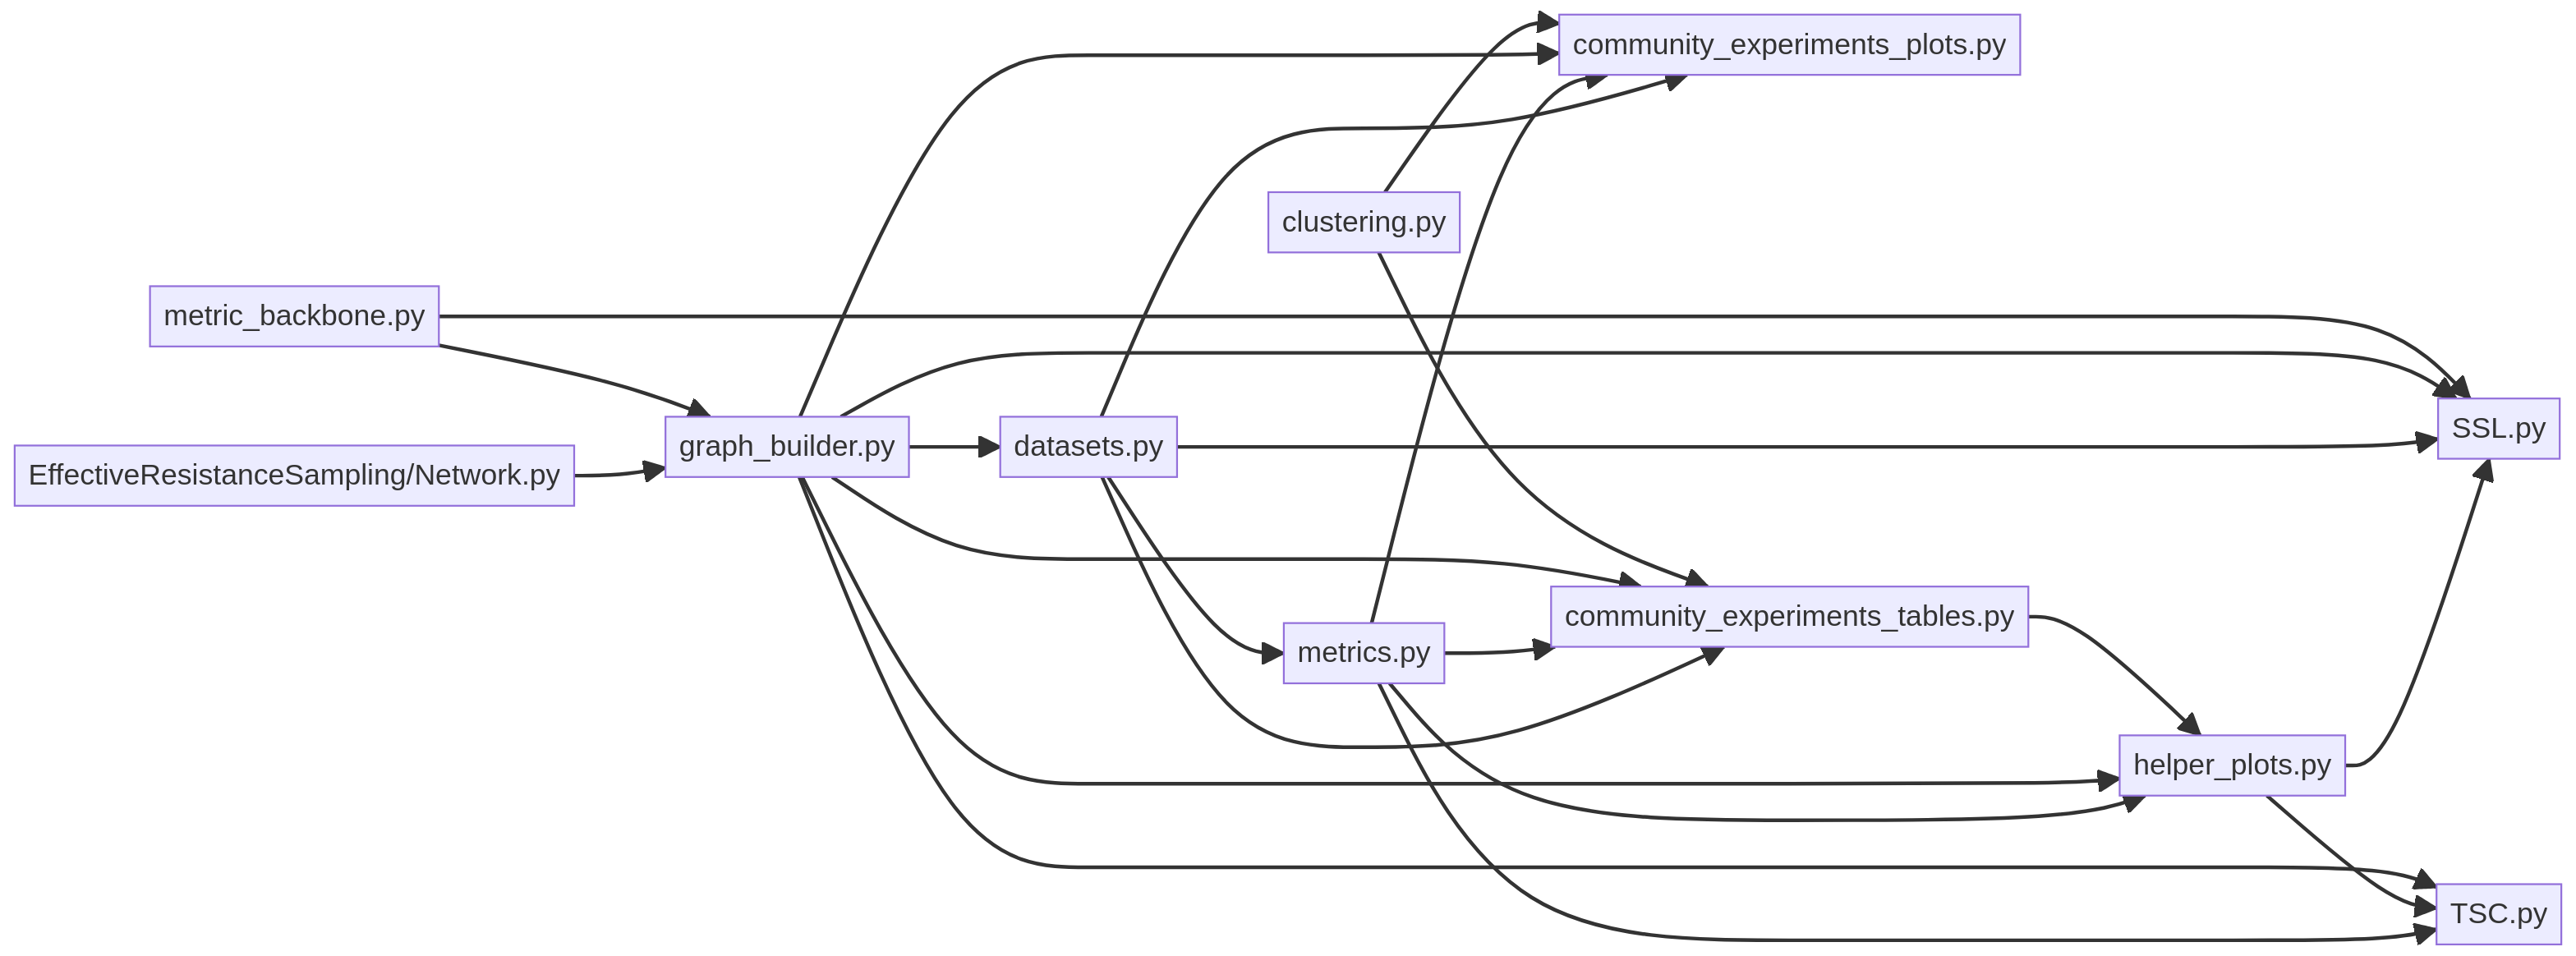
\includegraphics[width=14.69in,height=5.47in]{script_files/figure-latex/mermaid-figure-1.png}

\section{Abstract}\label{abstract}

\textbf{Introduction to Quarto and to a Measure-Theoretic First Passage
Percolation Framework for Inhomogeneous Random Graphs.}

\subsection{Row}\label{row-2}

Quarto documents are similar to Jupyter Notebooks, but better. They
allows one to centralize all ones work and to share it with the world
without having to establish a parallel workflow for presentation
preparation. In other words, your work is always ready to be shown. The
most obvious way in which Quarto does this is by building and deploying
an interactive website connected to your htlm-free code behind the
scenes. This allows anyone with a WiFi connection, to play with your
model's parameters and see the effects in real time. I will demonstrate
this and give a short tutorial for people who wish to use this exciting
tool.

I will be presenting the main ideas of Kolossváry's and Komjáthy's
``First Passage Percolation on Inhomogeneous Random Graphs (IHRG)''
paper. Here, ``Inhomogeneous'' refers to the fact that the edge
probabilities depend on the types of the end vertices in the model of
interest. The weighted stochastic block model (wSBM) can be seen as a
special case of an IHRG, so that all results from this paper remain true
for wSBMs. The authors of the paper strive to offer the most general
framework possible. In an applied setting, this should help us adjust
models serenely, knowing that no core properties will be lost.

\section{Quarto Tutorial}\label{quarto-tutorial}

\section*{Inhomogeneous Random
Graphs}\label{inhomogeneous-random-graphs}
\addcontentsline{toc}{section}{Inhomogeneous Random Graphs}

\phantomsection\label{refs}
\begin{CSLReferences}{1}{0}
\bibitem[\citeproctext]{ref-den2012probability}
Den Hollander, Frank. 2012. {``Probability Theory: The Coupling
Method.''} \emph{Lecture Notes Available Online (Http://Websites. Math.
Leidenuniv. Nl/Probability/Lecturenotes/CouplingLectures. Pdf)}.

\bibitem[\citeproctext]{ref-durrett2019probability}
Durrett, Rick. 2019. \emph{Probability: Theory and Examples}. Vol. 49.
Cambridge university press.

\end{CSLReferences}




\end{document}
